In most datasets, longer texts often result in higher classification performance.
So, an interesting question is whether the size of a concept map also correlates with its classification performance, ie. whether ``bigger" graphs in terms of the number of nodes and edges are easier to classify.
To test this, we classify the graphs with our standard approach, using the Weisfeiler-Lehman graph kernel, then a SVM to classify the feature maps.
For text, we extract the features with Tfidf-BoW, then also classify the features with a SVM.

% IGNORED
\iffalse
In the next step, we look at the results for different graph sizes, binning them with quantiles, in our case 10 quantiles, or deciles.

\begin{figure}[htb!]
    \begin{subfigure}[t]{.5\linewidth}  {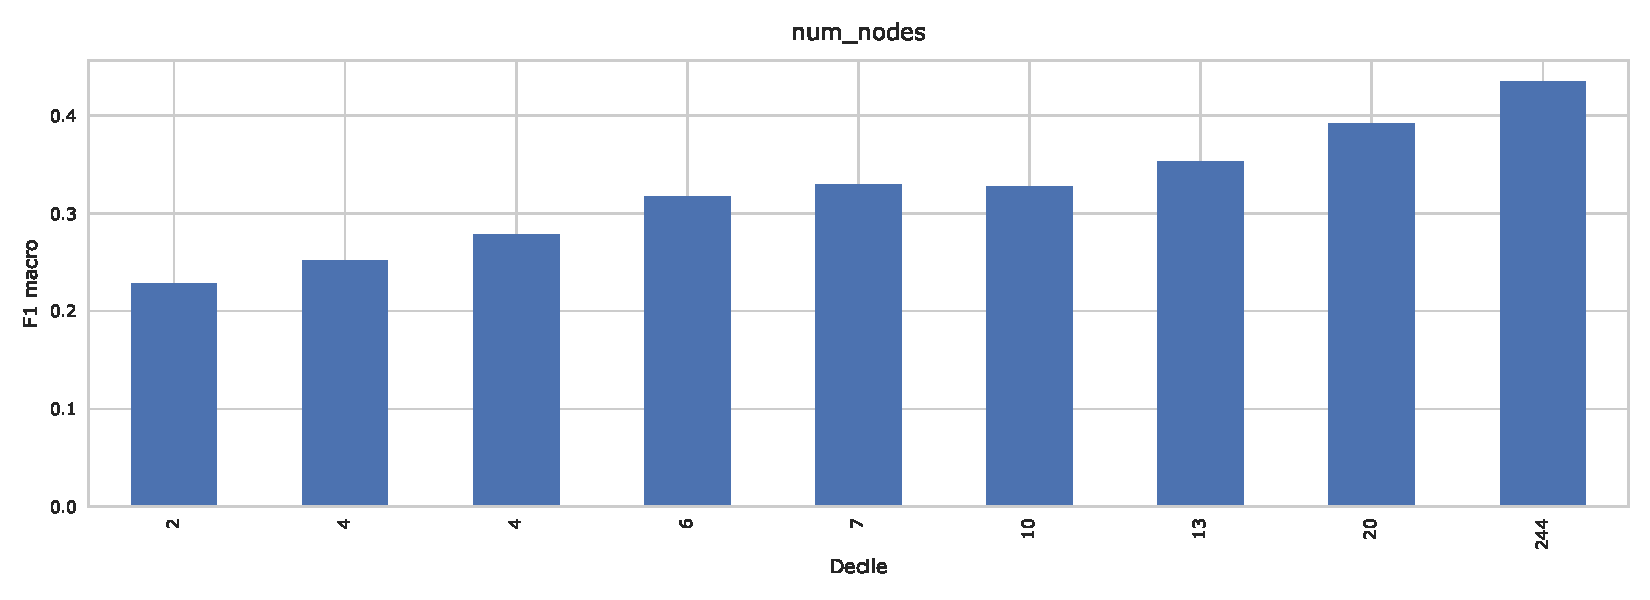
\includegraphics[width=\linewidth]{assets/figures/graph_binning_num_nodes.pdf}\label{fig:todo_1}}
    \caption{Graphs}
    \end{subfigure}
    \hfill
        \begin{subfigure}[t]{.5\linewidth}
    {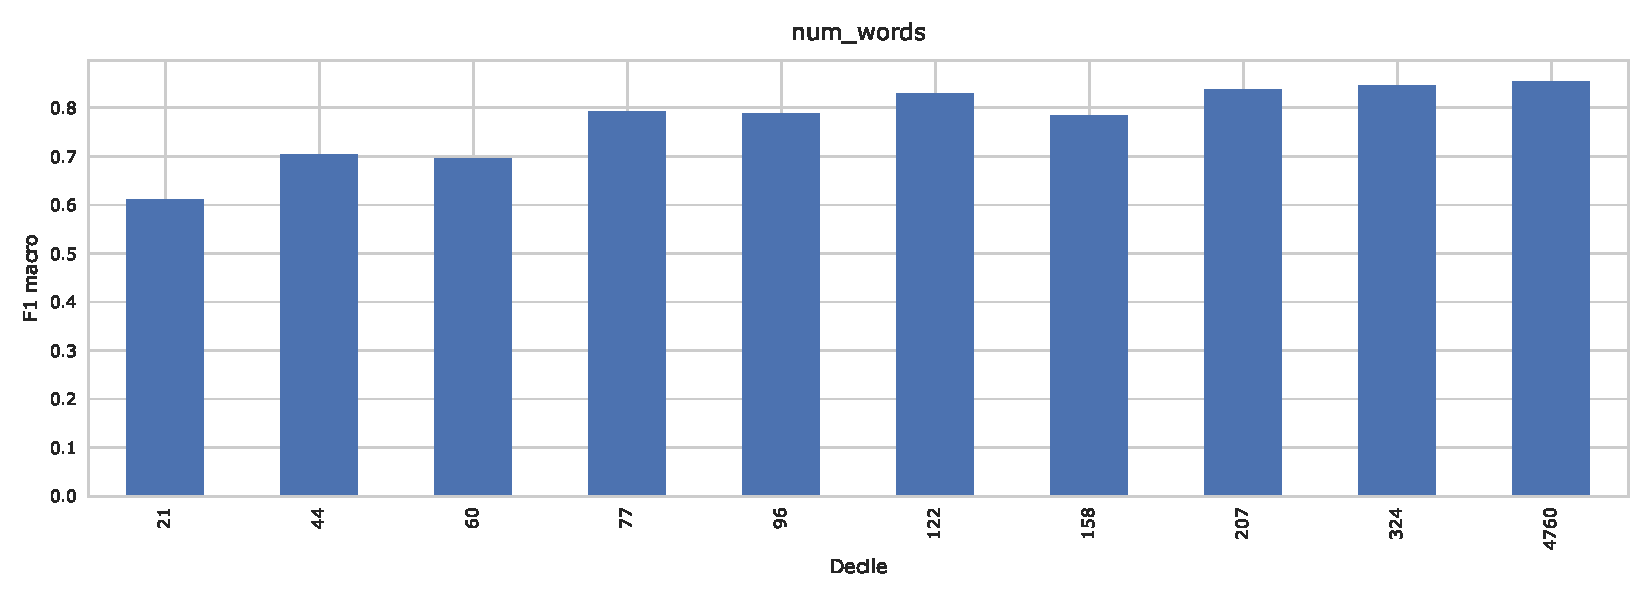
\includegraphics[width=\linewidth]{assets/figures/text_binning_num_words.pdf}\label{fig:todo_2}}
    \caption{Text}
    \end{subfigure}
    \caption[Statistics: Histogram of classification performance per graph/text size]{Classification performance per graph/text size. The x-axis corresponds to the size of the graph/text, the y-axis for the classification performance for graphs/text of that size. Dataset: \textit{ng20}}\label{fig:graph_size_performance}
\end{figure}


For the \textit{ng20} dataset, the results indicate that classification performance indeed correlates with the number of vertices.
In other datasets, this correlation is not as distinguished.
\fi

In Table \ref{table:correlations_size} we report the Spearman rank correlations \cite{Hauke2011} between the accuracy, ie. whether the label for the document/graph was predicted right, and the size of the document/graph.
Here, we also see a (weak) correlation for the graph sizes in some datasets.
In the \textit{ling-spam} and \textit{ng20} dataset, the accuracy correlates far more with the document/graph size than in other datasets.
It has to be noted that there is no partial similarity in accuracy, only 1 if the label was predicted right and 0 otherwise.
This might also explain that the relatively low correlation between the graph/document size and the accuracy, even in \textit{ng20}.

These results also highlights another finding: one observation for some dataset might not be consistent with observations from another dataset, eg. for our results the correlations are sometimes weak, sometimes practically not present at all.

We also tested other metrics to find correlations, for instance the number of edges or the number of connected components, yet we could not see relevant correlations.

\begin{table}[htb!]
    \centering
    \begin{tabular}{lrr}
\toprule
        &  \multicolumn{2}{c}{Spearman correlation} \\
        &  Graph &  Text \\
        \midrule
        ling-spam       &  0.2135 &  0.1490 \\
        ng20            &  0.2699 &  0.2415 \\
        nyt\_200         & -0.1986 &  0.0077 \\
        r8              & -0.0212 & -0.0499 \\
        review\_polarity & -0.0311 & -0.0286 \\
        rotten\_imdb     &  0.1680 &  0.0313 \\
        ted\_talks       & -0.0232 & -0.0991 \\
        \bottomrule
    \end{tabular}
    \caption[Table: Graph/text size correlations]{Spearman rank correlations between the accuracy and graph/text size. Here, the graph size is the number of nodes in the graph, text size the number of words. The higher the absolute value of the Spearman correlation is to 1, the higher the correlation.
    A positive correlation value between A and B means that if A increases, B also increases and vice versa.
    A negative correlation means that when A increases, B decreases and vice versa.}%
    \label{table:correlations_size}
\end{table}

\answersummary{
    In some datasets, we see a correlation between the size of graph/documents and the prediction accuracy.
    For other datasets, this correlation can not be measured distinctly.
    The results vary widely across datasets. 
}